\chapter{Grundlagen}\label{ch:grundlagen}
In diesem Kapitel werden für diese Arbeit wichtige Begriffe erläutert.

\section{Mainframe / Großrechner}\label{sec:mainframe}
Mainframe und Großrechner werden in dieser Arbeit gleichbedeutend verwendet.
Im modernen Sprachgebrauch kann ein Großrechner als größte zur Verfügung stehende Serverart betrachtet werden.
Er wird von Unternehmen verwendet, um  kommerzielle Datenbanken, Transaktionsserver und Anwendungen, die einen hohen Grad an Sicherheit und Verfügbarkeit benötigten, zu hosten.
Im Gegensatz zu verteilten Serversystemen, bei denen die Funktionalitäten auf einzelne Server, wie zum Beispiel einen E-Mail-Server, einen Datenbank-Server, einen Web-Server usw. aufgeteilt sind, handelt es sich bei einem Mainframe um ein zentralisiertes System.
Unter anderem sind Datenbanksysteme und Anwendungsserver sogenannte \glqq Subsysteme\grqq.
\cite{Ebbers.2011}

\subsection{Batch}
Batch beziehungsweise Batch-Verarbeitung bezeichnet in der IT die sog. \glqq Stapelverarbeitung\grqq.
Das heißt, dass Programme mit minimalem menschlichen Eingreifen nacheinander abgearbeitet werden.
Dies geschieht meist zu einer vorher festgelegten Zeit, gesteuert wird dies über sog. \glqq Scheduling\grqq-Systeme.
Zum Beispiel wird einmal am Tag zu einer ganz bestimmten Uhrzeit die tägliche Bewertung\footnote{Beschreibung in Absatz \ref{sssec:täglbew}} der DATEV Rechnungsschreibung durchgeführt.
Die auszuführenden Programme laufen in sogenannten \glqq Batch-Jobs\grqq.
\cite{Ebbers.2011}

\subsection{Batch-Job / Job}\label{ssec:job}
In einem Batch-Job, in dieser Arbeit wird \glqq Job\grqq{} gleichbedeutend verwendet, wird dem System mitgeteilt welches Programm mit welchen Ein- und Ausgabedateien und Parametern gestartet werden soll.
Die Skriptsprache, die diese Jobs definiert, ist im IBM-Mainframe-Umfeld die sog. \glqq Job Control Language\grqq, kurz JCL.
Die drei Grundbausteine der JCL werden im Folgendem beschrieben.

Zunächst ist \glqq JOB\grqq{} zu nennen, auch Jobkarte genannt.
Hier wird der Name des Jobs, Berechnungsinformationen, maximal zur Verfügung stehende CPU-Zeit und weitere Job-weite Parameter gesetzt.

Innerhalb eines Jobs wird mit Hilfe des \glqq EXEC\grqq{} Befehls dem System mitgeteilt, welches Programm gestartet werden soll.
Es können mehrere \glqq EXEC\grqq{}  Befehle in einem Job vorkommen, dabei wird jeder einzelne als sogenannter \glqq Job step\grqq{} bezeichnet.
Dabei können dem Programm neben den Ein-/Ausgabedateien auch weitere Parameter übergeben werden.

Als letztes ist der \glqq DD\grqq{} Baustein zu nennen.
\glqq DD\grqq{} steht für Data Definition.
Ein DD-Statement verknüpft den sog. DD-Namen mit einer Datei oder einem I/O Gerät und ist somit ein Alias für diese.
Ein \glqq DD\grqq{} Baustein ist immer an ein \glqq EXEC\grqq{} Befehl gebunden.
Einem \glqq EXEC\grqq{} können mehrere \glqq DD\grqq{} Bausteine zugeordnet sein. 
\cite{Ebbers.2011}

\subsection{Resource Access Control Facility}
Die Resource Access Control Facility, kurz RACF, ist ein externer Sicherheitsmanager für z/OS.
Dieser bietet eine Rechteverwaltung für das z/OS Betriebssystem an.
Damit werden unter anderem Zugriffsrechte auf Dateien und Subsysteme gesteuert.
\cite{InternationalBusinessMachinesCorporation.2008}

\subsection{REXX}
Die Restructures Extenden Executer Programmiersprache, kurz REXX, ist eine prozedurale Programmiersprache.
Die Sprache wird interpretiert.
Mittlerweile existieren jedoch auch REXX-Compiler.
\cite{Parziale.2007}

REXX versteht sich als Skriptsprache und kommt nicht nur am Mainframe zum Einsatz.
So kann es als Bindeglied für Betriebssystembefehle, grafischen Interfaces, Objekten, Funktionen und Serviceroutinen gesehen werden.
So wird es, wie auch in dieser Arbeit, unter anderem für die Automation von sich wiederholenden Systemadministrations Aufgaben eingesetzt.
\cite{Fosdick.2005}

\section{IBM Mainframe Architektur bei der DATEV eG}
Folgende Begriffe werden in diesem Absatz im Umfeld der DATEV eG erläutert:

\begin{samepage}
\begin{itemize}
\item Stages, Sysplexe und Logical Partitions
\item Middleware / Subsysteme
\item Architekturüberblick
\end{itemize}
\end{samepage}

Die DATEV eG bezogenen Informationen stammen aus Gesprächen mit Mitarbeitern der einzelnen Administratorenteams.

\subsection{Stages, Sysplexe und Logical Partitions}\label{sec:sysplex}
Innerhalb der DATEV eG existieren vier sogenannte \glqq Stages\grqq{} auf dem Mainframe.
Dabei handelt es sich um abgekapselte Systemumgebungen.
Eine Stage besteht aus einer oder mehreren \glqq Logical Partitions \grqq, kurz LPARs, mit eigenen Subsystemen und eigener Ressourcenverwaltung. 
Zu den Subsystemen zählen unter anderem CICS \footnote{Beschreibung in Absatz \ref{cics}},  Db2\footnote{Beschreibung in Absatz \ref{sssec:db2}} und IBM MQ\footnote{Beschreibung in Absatz \ref{sec:mq}}.
Dadurch wird eine strickte Trennung zwischen den Stages realisiert.
Die vier Stages werden im Folgenden beschrieben.

\subparagraph{\glqq Entwicklung\grqq}~\\
Stage auf der alle z/OS Entwickler an neuen Features arbeiten und erste kleinere Tests durchführen.

\subparagraph{\glqq Qualitätssicherung\grqq} ~\\
Hier werden vor allem Integrationstests mit extra dafür erstellen Testdaten durchgeführt.

\subparagraph{\glqq Vorproduktion\grqq}~\\
Die Vorproduktion steht für weitere Integrationstests zur Verfügung.
Jedoch produktionsnäher und auch mit Echtdaten, also Daten aus der Produktion.

\subparagraph{\glqq Produktion\grqq}~\\
Hier befindet sich die Software, die von den Kunden verwendet wird.
Ein Programm muss die Entwicklungs-, Qualitätssicherungs- und Vorproduktionsstages durchlaufen bevor es dem Kunden in der Produktion zur Verfügung gestellt wird.

Die LPARs der vier Stages sind auf zwei sogenannte  \glqq Sysplexe\grqq{} aufgeteilt.
Ein Sysplex kümmert sich um die Kommunikation zwischen den LPARs der einzelnen Stages und verwaltet Ressourcen LPAR übergreifend.
\cite{Kyne.2016}

Neben den oben erwähnten zwei Sysplexen existiert noch ein weiterer Sysplex.
Diese werden alle im Folgenden beschrieben.

\subparagraph{\glqq LAB/Test-Plex\grqq}~\\
Der Test-Plex ist als Labor für Änderungen am System zu betrachten.
So werden zum Beispiel neue Betriebssystemsversionen auf diesem geprüft.

\subparagraph{\glqq QS-Plex\grqq}~\\
Enthält unter anderem die LPARs der Entwicklung und der Qualitätssicherung.

\subparagraph{\glqq Prod-Plex\grqq}~\\
Im Prod-Plex sind die LPARs der Vorproduktion und der Produktion enthalten.

\subsection{Middleware / Subsysteme}
In diesem Absatz wird die verwendete Middleware beziehungsweise die verwendeten Subsysteme beschrieben.
Diese setzen auf dem IBM Mainframe Betriebssystem z/OS auf.

\subsubsection{Customer Information Control System}\label{cics}
Das Customer Information Control System, kurz CICS, ist ein Applikationsserver für einen IBM-Großrechner mit Betriebssystem z/OS und damit eine IBM Middleware.
Ein Applikationsserver stellt eine Umgebung zur Verfügung, in der Anwendungen gehostet werden können.
Dabei kümmert sich dieser unter anderem um Transaktionalität, Webkommunikation und Sicherheit.
Hierfür stellen Applikationsserver eine API zur Verfügung.
CICS hat einen Vorteil gegenüber anderen Anwendungsservern, es unterstützt verschiedene Programmiersprachen.
CICS ist ein Multi-Language Application Server und unterstützt z.B. COBOL, Assembler, Java und PLI.
So können Programme innerhalb einer Anwendung in der für ihren Use-Case am besten geeigneten Sprache implementiert werden.
\cite{Rayns.2011}

Das CICS Subsystem einer Stage umfasst mehrere CICS Instanzen.

\paragraph{CICS Instanz} ~\\
Unter einer CICS Instanz ist ein einzelner Bereich, der auf dem z/OS Kernel aufsetzt, zu verstehen.
Dieser Bereich ist mittels einer eindeutigen CICS ApplicationID gekennzeichnet und kann darüber explizit angesprochen werden.
Eine CICS Instanz verwaltet mehrere CICS Transaktionen.

Wenn in dieser Arbeit von dem CICS gesprochen wird, ist die CICS-Instanz damit gemeint.

\paragraph{CICS Transaktion}\label{subsec:trans} ~\\
Ein Businessablauf wird im CICS in einer Transaktion gekapselt.
Eine Transaktion kann mehrere Programme unterschiedlicher Programmiersprachen umfassen und wird über eine eindeutige \glqq TransaktionsID\grqq{} identifiziert..

Über die TransaktionsID wird der Ablauf gestartet.
Dies kann sowohl per Webanfrage oder per Messaging Queue als auch aus einem anderen Programm heraus oder manuell geschehen.
In der Transaktion werden alle Änderungen, die Programme an Ressourcen, wie zum Beispiel einer Datenbank oder Dateien tätigen, protokolliert.
So wird im Fehlerfall die Möglichkeit eines Rollbacks sichergestellt.
 \cite{Rayns.2011}

\paragraph{Voraussetzungen}\label{subsec:voraus} ~\\
Bei der DATEV eG kümmert sich ein Team, die \glqq CICS Administration\grqq{} um das Erstellen einer CICS-Instanz, starten dieser Instanz und ist generell für alles rund um die Administration des CICS Transactions Servers zuständig.
Der Fokus dieser Arbeit liegt auf dem Erstellen (\glqq Provisionieren\grqq{}) einer CICS-Instanz. Es werden nur die dafür notwendigen Voraussetzungen dargelegt.
Außerdem liegt der Fokus auf Entwicklungs-CICS-Systemen, auf der sog. Entwicklungs-Stage, nicht auf den produktiven CICS-Systemen der DATEV eG. 
Aus diesem Grund werden nur Schritte, die für ein solches Testsystem benötigt werden, dargestellt.
Eine weitere Rahmenbedingung besteht darin, dass nur die Arbeitsschritte, die mit z/OSMF\footnote{Beschreibung in Absatz \ref{sec:zosmf}} automatisiert werden, erläutert werden.

\paragraph{Einrichtung CICS Instanz}\label{subsec:createCICS}~\\
Die in diesem Absatz benötigten Informationen stammen aus Gesprächen mit Mitarbeiter 2 aus der Abteilung, die für die CICS Administration zuständig ist.
Um eine lauffähige CICS Instanz den Vorausetzungen aus dem Absatz \ref{subsec:voraus} entsprechend einzurichten, sind mehrere Schritte notwendig.
Diese werden im Folgendem beschrieben.

\subparagraph{CICS spezifische Dateien}\label{sssec:speziDat} ~\\
Zunächst müssen CICS spezifische Dateien im z/OS angelegt werden.
Im Fall des dieser Arbeit zugrunde liegende Beispiels handelt es sich um 17 verschiedene VSAM\footnote{Virtual Storage Access Method, spezielle Dateiart, die schnelle I/O-Zugriffe ermöglicht.\cite{Lovelace.2013}} Dateien.
Diese Dateien benötigt die CICS Instanz um zum Beispiel Systemfehler zu protokollieren oder den Debugger aktivieren zu können.

\subparagraph{CSD} ~\\
In der Datei \glqq CICS System Defintion\grqq, kurz CSD, muss jede Ressource, die dem System zur Verfügung stehen soll, definiert werden.
Eine CSD Datei kann für mehrere CICS Instanzen verwendet werden.
Eine CSD Datei besteht aus mehreren Einträgen.
Ein Eintrag besteht aus einer Gruppe und einer Liste.
Die Gruppe ist hierbei die Definition einer Systemressource und muss manuell angelegt werden.
Bei der Liste handelt es sich um das System, welches diese Ressource benötigt.
Dort ist unter anderem für jede CICS Instanz hinterlegt, zu welchem Db2 Datenbanksystem und welchem IBM MQ Messagingsystem sich diese Instanz verbinden soll.

\subparagraph{STC Job} ~\\
Bei einem Started Task Control-Job, kurz STC Job, handelt es sich um einen Batch Job, der mit Hilfe des \glqq START\grqq-Konsolenkommandos innerhalb von z/OS gestartet werden kann.
Dieser Batch Job wird deshalb auch als Started Task bezeichnet.\cite{Cassier.2007}
Bei der DATEV eG existiert für jede Instanz eines Subsystems ein solcher Job, so also auch für CICS.
In diesem werden zunächst einige zur Laufzeit benötigten Bibliotheken und Dateien eingebunden, unter anderem die CICS spezifischen Dateien\footnote{Beschreibung in Absatz \ref{sssec:speziDat}}.
Außerdem werden hier die SIT \footnote{CICS system initialization table} Parameter definiert.
Zunächst wird festgelegt welche Standard SIT verwendet werden soll.
Anschließend können diese Standardwerte überschrieben werden.
Zu diesen Parameter zählen unter anderem der eindeutige Name der CICS Instanz, der Speicherort der dazugehören CSD und die Information, ob eine Verbindung zu einem Db2 Datenbanksystem hergestellt werden soll.

\paragraph{Entfernung CICS Instanz} ~\\
Um eine CICS Instanz zu entfernen muss diese zunächst gestoppt werden.
Dies ist über das \glqq STOP\grqq-Konsolenkommando von z/OS möglich.
Anschließend müssen alle im Absatz \ref{subsec:createCICS} beschriebene Schritte rückgängig gemacht werden.
Also müssen die für diese Instanz spezifischen Dateien, die Einträge für die CICS Instanz aus der CSD Datei und schließlich auch der STC Job gelöscht werden.

\subsubsection{Db2}\label{sssec:db2}
Db2 ist ein relationales Datenbanksystem, welches unter anderem als Subsystem eines z/OS Betriebssystems läuft.
Einer Stage können mehrere Datenbanksysteme, auch Instanz genannt, zugeordnet werden.
In diesem befinden sich die Datenbanken und Tabellen.

\subsubsection{IBM MQ}\label{sec:mq}
IBM MQ ist eine Messaging-Lösung der IBM.
Diese ermöglicht den asynchronen Datenaustausch zwischen Anwendungen mittels sogenannter Queues.
Alle IBM MQ Begrifflichkeiten, die in dieser Arbeit verwendet werden, werden im Folgenden erläutert.
\cite{Aranha.2013}

Das IBM MQ Subsystem einer Stage setzt sich aus einem oder mehreren Queue Managern zusammen.
Ein Queue Manager kann so als IBM MQ Instanz gesehen werden.

\paragraph{Queue Manager}~\\
Bei einem Queue Manager handelt es sich um die zentrale Ressource eines IBM MQ Systems.
Er verwaltet  alle anderen IBM MQ Ressourcen.
Dazu gehören unter anderem die Speichersteuerung der Daten und die Wiederherstellung dieser im Falle eines Fehlers.
Desweiteren koordiniert er den Zugriff aller Anwendungen auf die Nachrichten in den von ihm verwalteten Queues.
Um hierbei die Konsistenz sicherzustellen, sorgt er für Locking und die notwendige Isolation der Queues.
\cite{Aranha.2013}

\paragraph{Queues}~\\
In Queues werden die Nachrichten, die von Programmen gesendet und gelesen werden gespeichert.
Es gibt verschiedene Arten von Queues, die im Kontext dieser Arbeit relevanten Queues sind folgende:

\subparagraph{Die Local Queue.}~\\
Dabei handelt es sich um die einzige Queue Art, bei der die Nachrichten physikalisch gespeichert werden.
Die anderen Queue Arten nutzen als Basis immer eine Local Queue.

\subparagraph{Initiation Queue}~\\
Die sogenannte \glqq Initiation Queue\grqq{} ist eine spezielle Art der Local Queue.
Diese dient dem Queue Manager dazu, um unter bestimmten Bedingungen eine Trigger-Nachricht darauf zu schreiben.
So kann eine andere Local Queue so definiert sein, dass sobald eine Nachricht auf sie geschrieben wird eine solche Trigger-Nachricht erzeugt wird.
Dies ermöglicht, dass Anwendungen nur starten, wenn wirklich Daten zum Verarbeiten vorhanden sind.
\cite{Aranha.2013}

\paragraph{Process}~\\
Für das Auslösen von Anwendungen wird nicht nur die Initiation Queue benötigt, sondern auch sogenannte \glqq Processes\grqq.
So muss der Local Queue, die den Start einer Anwendung auslösen soll, bei der Definition nicht nur die Initiation Queue bekannt gemacht werden, sondern auch ein Process.
Ein Process legt den \glqq Type\grqq{} und den Namen der zu startenden Anwendung fest.
Als \glqq Type\grqq{} können beispielhaft CICS oder auch WINDOWSNT für Windows unterstütze Platformen genannt werden.
Ist der \glqq Type\grqq{} CICS,  muss der Name der Transaktion angegeben werden, für Windows Platformen der Dateipfad der auszuführenden exe.
\cite{Aranha.2013}

\subsection{Architekturüberblick}
In Abbildung \ref{fig:archüber} sind die einzelnen Subsysteme mit ihren Instanzen dargestellt.
Als Grundbaustein dient allen der z/OS Kernel.

\begin{figure}[h]
\centering
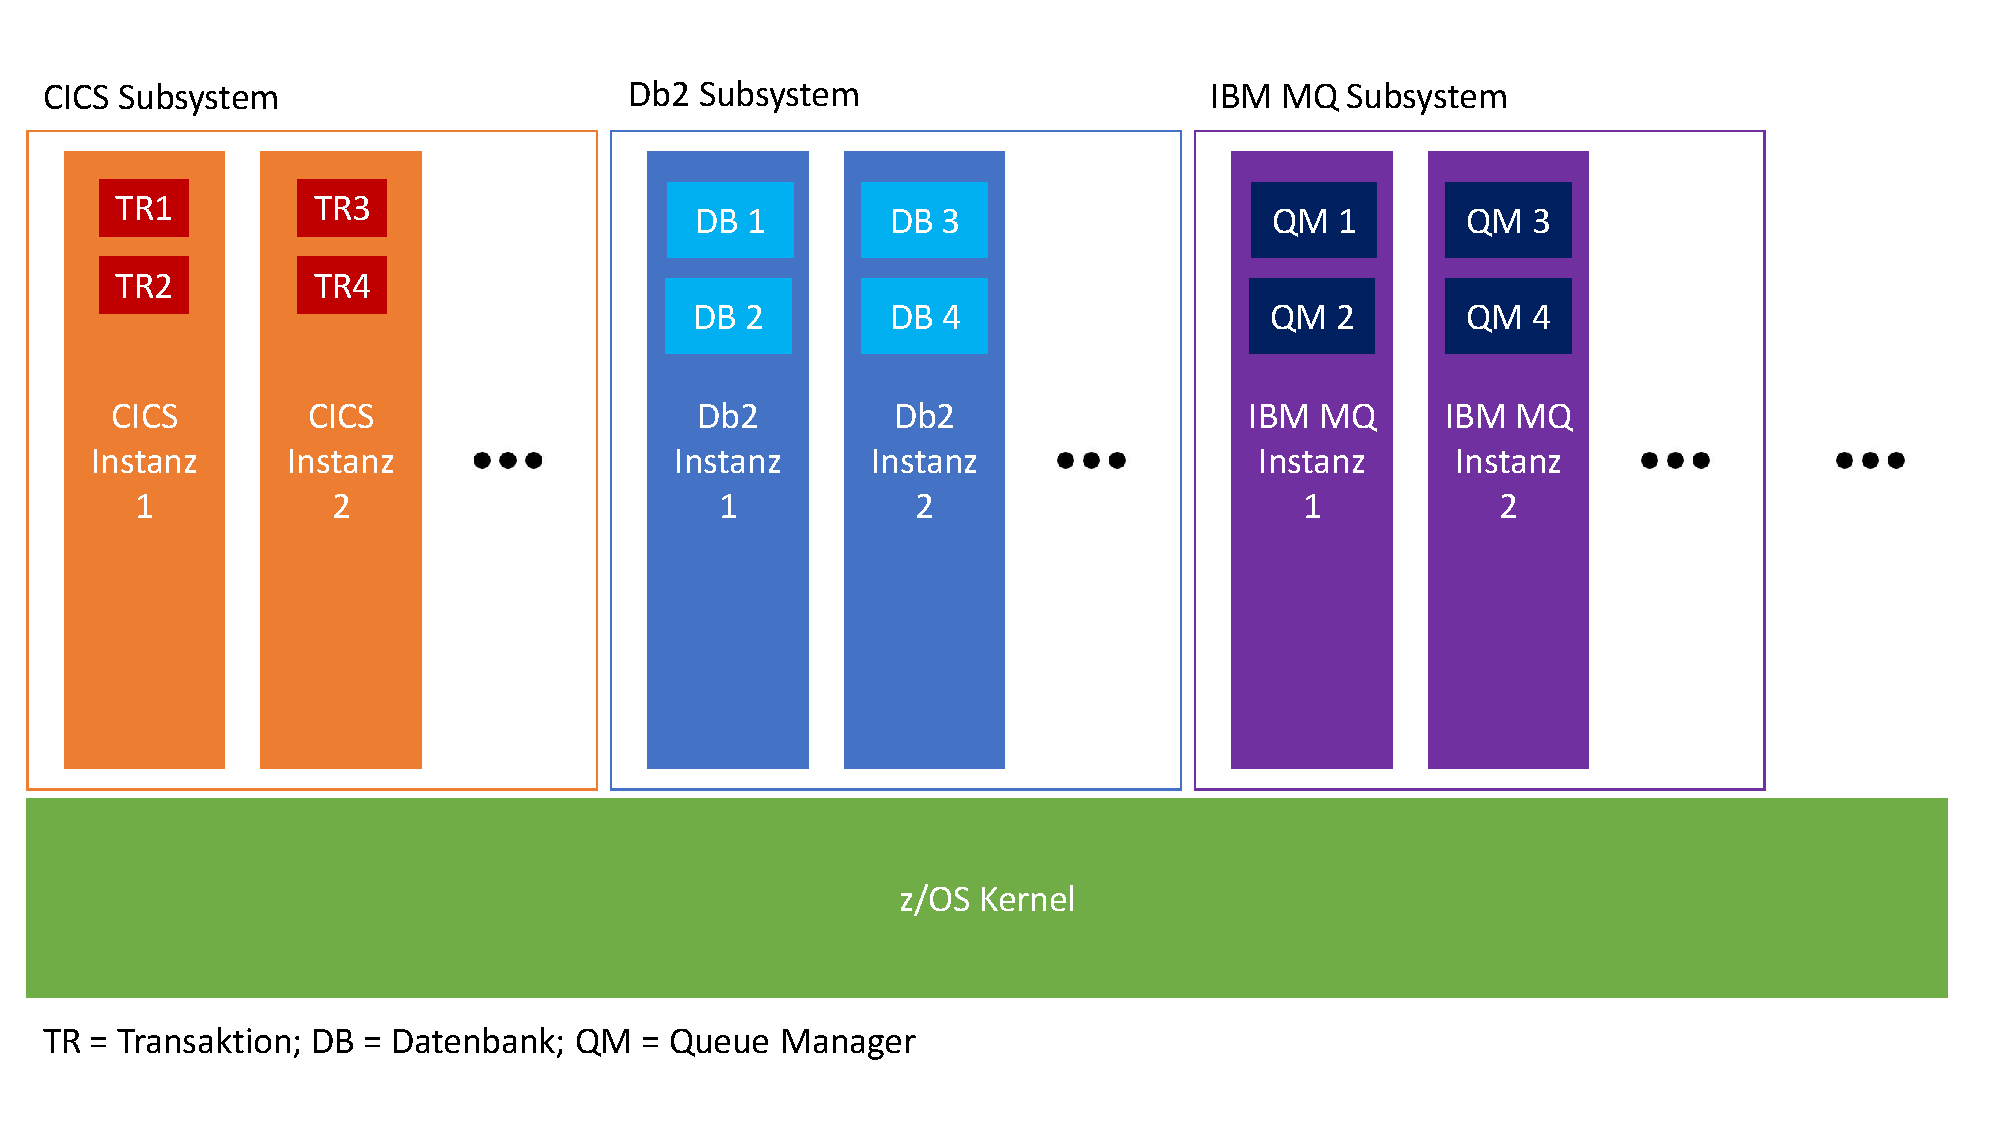
\includegraphics[width=\textwidth]{figures/architektur.pdf}
\caption{Architekturübersicht über die Subsysteme bei DATEV eG}
\label{fig:archüber}
\end{figure}

\section{IBM Cloud Provisioning and Management for z/OS}\label{sec:zosmf}
In diesem Absatz wird zunächst auf die für dieses Kapitel grundlegenden Begriffe eingegangen.
Das IBM Cloud Provisioning and Management for z/OS bietet die Möglichkeit, mehrere Systeme (sog. Middleware) innerhalb eines z/OS Betriebssystems zu provisionieren, unter anderem Laufzeitumgebungen wie CICS. 
Für diese Aufgaben stehen zwei Schnittstellen zur Verfügung.
Zum einen das z/OS Provisioning Toolkit, (z/OSPT) und zum anderen z/OS Management Facility (z/OSMF).
\cite{KeithWinnardGaryPuchkoffHirenShah.2016}

\subsection{Begrifferklärung}
Im Folgenden werden einige allgemeine Begriffe, die im Umfeld des Tools \glqq IBM Cloud Provisioning and Management for z/OS\grqq{} vorkommen, erläutert.

\subsubsection{Provisioning}
Ins Deutsche übersetzt bedeutet es Bereitstellung, in dieser Arbeit wird auch Provisionierung verwendet.
In dieser Arbeit umfasst dieser Begriff die Bereitstellung einer Laufzeitumgebung, beziehungsweise den Prozess, der hierfür benötigt wird.

\subsubsection{Workflow}\label{sssec:workflow}
Ein Workflow ist eine beliebig komplexe, eindeutige Aneinanderreihung von sogenannten Steps.
Nach der Ausführung dieser Steps wird ein bestimmtes Ziel erreicht, zum Beispiel die erfolgreiche Bereitstellung eines CICS Systems.
Für die Definition eines Workflows, der dazugehörigen Steps und ihrer Variablen wird XML genutzt.
Ein Step beschreibt einen Teilablauf eines Workflows.
Innerhalb eines Steps können sowohl interne und externe Scripte als auch JCLs und somit Programme ausgeführt werden.
Darüber hinaus besteht die Möglichkeit REST-Calls auszuführen.
Es können Bedingungen für die Durchführung eines Steps definiert werden.
So ist es zum Beispiel möglich, einen Step nur durchzuführen, wenn eine bestimmte Variable einen bestimmten Wert besitzt.
Es wird ein XML Schema verwendet um sicherzustellen, dass in dem XML-Skript zur Laufzeit keine syntaktischen Fehler vorhanden sind.
\cite{Rotthove.2018}

Ein Nachteil von Workflows ist, dass diese statisch sind, das heißt, dass die Variablenzuweisungen immer zum Zeitpunkt der Erstellung stattfindet.
Dadurch ergibt sich, dass für jede kleine Änderung ein eigener Workflow erzeugt werden muss.
Somit ist ein Workflow eher ein Einmal- bzw. Wegwerfprodukt.

\subsubsection{Template}
Bei dem Nachteil von Workflows als Wegwerfprodukt setzen die sogenannten Templates an.
Ein Template besteht aus drei Dateien.

\begin{enumerate}
\item Datei für Eingabevariablen.\\
In dieser Datei kann Workflowvariablen Werte zugewiesen werden.
Diese Variablen müssen bei ihrer Definition im Workflow entsprechend gekennzeichnet sein.

\item Die sogenannte Aktion-Definitions-Datei.\\
Hier werden die Aktionen, die ein Anwender mit diesem Template durchführen kann, festgelegt.
Einer Aktion wird eine Workflow Definitions Datei und somit ein Workflow zugewiesen.
Darin ist die Datei für die Eingabevariablen und die Festlegung, welche Variablen davon verwendet werden, anzugeben.

\item Die Manifest-Datei.\\
In dieser wird dem Template mitgeteilt, an welchem Speicherort sich die oben genannten Dateien befinden.
Da ein Template immer provisioniert werden kann, wird hier auch der Speicherort des Bereitstellungsworkflows angeben.
Zusätzlich kann noch eine Beschreibung des Templates hinzugefügt werden.
\end{enumerate}

Somit bildet ein Template einen Rahmen um mehrere Workflows und ermöglich eine schnellere De-/provisionierung.
Das hat den Vorteil, dass Variablen nur an einer Stelle geändert werden.
Daüber hinaus besteht die Möglichkeit, per Awendereingabe den Variablen zum Zeitpunkt der Provisionierung einen Wert zuzuweisen.
Somit ist ein Template deutlich flexibler als ein Workflow.
\cite{IBM.2019}

\subsubsection{Instance}\label{sssec:instance}
Hierbei handelt es ich um das Ergebnis nach der Provisionierung eines Templates, zum Beispiel um ein funktionsfähiges CICS.
Als Abgrenzung zu einer Instanz eines Subsystems, kann eine Template Instance auch Instanzen mehrer Subsystemen enthalten.

\subsection{z/OS Provisioning Toolkit}\label{sssec:zospt}
z/OSPT bietet ein Kommandozeileninterface für die Bereitstellung und das Verwalten von Laufzeitumgebungen.
In Abbildung \ref{fig:zospt_help} werden die möglichen Kommandozeilenbefehle mittels des Befehls \glqq zospt -h\grqq{} in einem Kommandofenster angezeigt.
\begin{figure}[h]
	\centering
	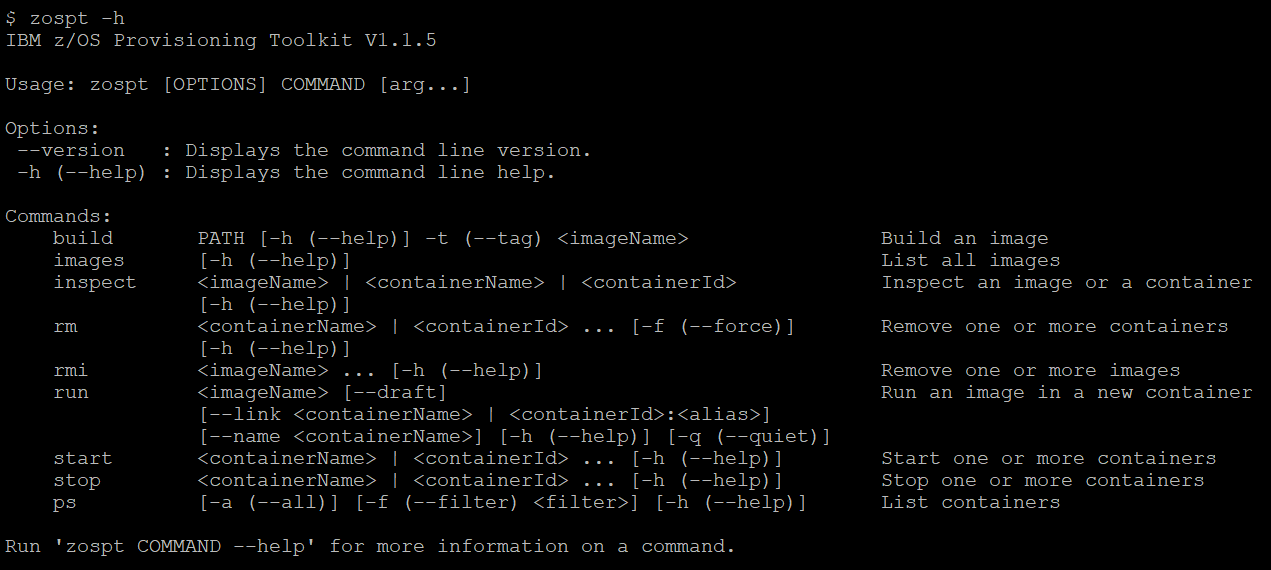
\includegraphics[width=\textwidth]{figures/zospt_help_putty.png}
	\caption{z/OSPT mögliche Kommandozeilenbefehle}
	\label{fig:zospt_help}
\end{figure}
Mit z/OSPT werden noch zwei weitere Begriffe eingeführt.\\
\glqq Images\grqq{}.
Dabei handelt es sich grundsätzlich um ein Template, jedoch kann dieses Template über eine weitere Inputdatei verändert werden.
Dadurch kann ein Template mit spezifischen Änderungen provisioniert werden, ohne dass ein neues Template erzeugt werden muss.
Dies erhöht die Flexibilität der Templates weiter.

\glqq Container\grqq{}.
Dabei handelt es sich eins zu eins um eine \glqq Instance\grqq \footnote{Beschreibung in Absatz \ref{sssec:instance}}.
\cite{IBM.2019b}

\subsection{z/OS Management Facility}\label{sssec:zosmf}
Der Hauptaugenmerk dieser Arbeit liegt  bei z/OSMF, da damit die Verwaltung von Workflows und Templates über eine browserbasierende Schnittstelle möglich ist.
Durch diese Oberfläche, in Abbildung \ref{fig:zosmf_welcome} dargestellt, ist es einfacher zu bedienen als das Kommandozeileninterface von z/OSPT  und somit wird der Einstieg in die Provisionierung erleichtert.

//hier zosmf welcomepage screenshot

Die linke Seite der Abbildung \ref{fig:zosmf_welcome} zeigt den Umfang der z/OSMF  Funktionen.
Für diese Arbeit besitzt nur der Menüpunkt \glqq Cloud Provisioning\grqq{} Relevanz.
Unter diesem Punkt sind die Funktionalitäten für die automatisierte Bereitstellung von Templates zu finden.
\cite{Rotthove.2018}

Zuerst ist das \glqq Resource Management\grqq{} zu nennen..
Darunter werden sogenannte \glqq Domains\grqq{} und die dazugehörigen \glqq Tenants\grqq{} verwaltet.
Unter einer \glqq Domain\grqq{} ist ein System zu verstehen, das Systemressourcen in Ressourcenpools gliedert.
\glqq Tenants\grqq{} sind die dazugehörigen Rechtegruppen, die dem Anwender den Zugriff auf und die Nutzung von zugeordneten Templates ermöglicht.
Einem Template muss sowohl eine\glqq Domain\grqq{} als auch ein \glqq Tenant\grqq{} zugewiesen werden.
\cite{Rotthove.2018}

Zur Verwaltung der Templates und Instances kommen die \glqq Software Services\grqq{} zum Einsatz.
Dort können neue Templates über die \glqq Manifest Datei\grqq{} hinzugefügt werden.
Dann muss, wie oben beschrieben, eine \glqq Domain\grqq{} und ein \glqq Tenant\grqq{} zugwiesen werden.
Anschließend kann das Template, falls es keine Fehler beinhaltet, veröffentlicht werden.
Es ist zu empfehlen vorher einen \glqq Test Run\grqq{} durchzuführen.
Dabei wird eine Instance testweise provisioniert.
Diese Instance verhält sich genauso wie eine Instance, die aus einem veröffentlichten Template erzeugt wurde.
Somit können damit das Template und die in der Aktion-Definitions-Datei definierten Aktionen getestet werden.
\cite{Rotthove.2018}
